\chapter{Metodologia}
\label{chap:MatMet}

O Capítulo \ref{chap:FUNDA} apresentou alguns dos métodos encontrados na literatura para a representação computacional de formas a partir do contorno.  Em muitos casos, esses métodos apresentam parâmetros que requerem ajustes dependentes da natureza da aplicação, ou seja,  das características da base de imagens e o propósito ao qual o sistema de reconhecimento se destina. A energia de dobramento multiescala, por exemplo, requer o ajuste do número e dos valores das escalas utilizadas na representação das formas. 
Esse capítulo apresenta um método que permite customizar descritores multiescala à base de imagens de formas melhorando o desempenho em classificação supervisionada e não supervisionada. 
\textcolor{red}{
Iniciamos este capítulo apresentando, em linhas gerais, o método proposto (Sessão \ref{sec:met}). Nas sessões subsequentes detalhamos cada etapa envolvida no processo de customização do descritor. 
}

\section{Customização de descritores\label{sec:met}}
O método para customização de descritores segue o esquema da Figura \ref{fig:Avaliacao}. O objetivo dessa metodologia é melhorar a representação do descritor de formas ajustando seus parâmetros através de algoritmos de otimização evolutivos. Foi utilizada como função objetivo na otimização o \ac{MAD} da métrica de avaliação de agrupamentos \textit{silhouette} \cite{Rousseeuw:1987}. O que motivou a escolha dessa função objetivo é sua robustez a \textit{outliers} \cite{Rousseeuw:1987:2}, sendo sua equação definida por

\begin{equation}
\label{eq:mad}
MAD = \operatorname{mediana}\big(|s_i - 1|_{i =1,\:2,\:\cdots,\:L}\big)\text{,}
\end{equation}

\begin{figure*}[ht]
\caption{\label{fig:Avaliacao}
 Proposta de uma metodologia para otimização evolucionária de um descritor multiescala de forma.} 
\centering
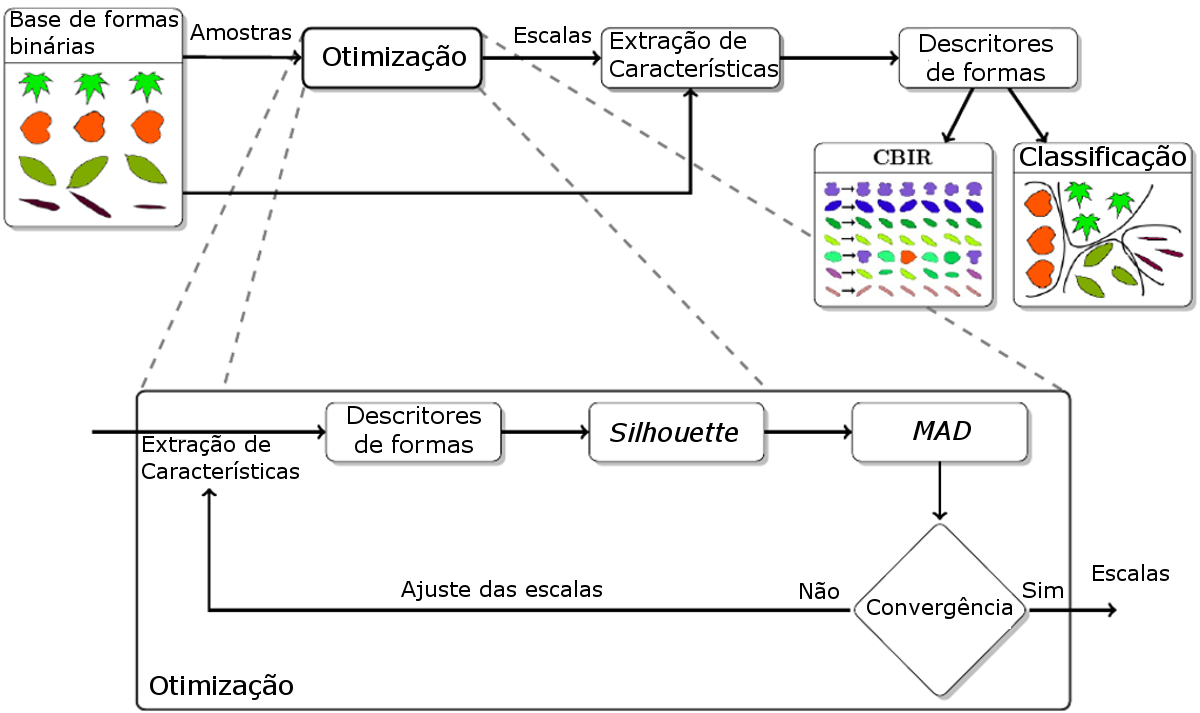
\includegraphics[width=\textwidth]{finalFlux1.jpg}
\end{figure*}

\noindent sendo $S = \{s_1,s_2,\cdots,s_L\}$ é o conjunto das \emph{silhouettes} calculadas para $L$ descritores de forma. Os operadores $|.|$  e {$mediana ( )$} retornam o valor absoluto e a mediana de um conjunto de valores, respectivamente.

A \textit{silhouette }\cite{Rousseeuw:1987} é uma medida de qualidade de agrupamentos que indica o grau de afinidade de uma amostra  a um agrupamento, considerando as distâncias médias entre classes e intra classes de um objeto $i$ atribuído a uma dada classe $A$. Logo, esta métrica é definida como 
\begin{equation}
s_i = \frac{b_i - a_i}{\max{(a_i,b_i)}} \in [-1,1],
\end{equation}

\noindent sendo $a_i$ a dissimilaridade média entre o objeto $i$ e os demais objetos pertencentes a mesma classe de $a_i$ e $b_i$ é a dissimilaridade média do objeto $i$ e a classe vizinha mais próxima de $i$, excluída sua própria classe. 

Essa métrica pode assumir valores no intervalo $[-1,1]$, sendo que valores negativos indicam que o grau de pertencimento de um objeto à classe que este fora atribuído é baixo. Já valores positivos indicam que o grau de pertencimento de um objeto à classe que este fora atribuído é alto. Um valor de \textit{silhouette} próximo de zero indica que o objeto está na fronteira entre duas classes e que há, portanto, um grau de incerteza a respeito de qual classes este pertence.

A função objetivo \ac{MAD} assume valores no intervalo $[0,2]$. De forma análoga à \textit{silhouette}, um valor igual a zero indica que a estrutura dos agrupamentos é perfeita, enquanto que valores próximos de $2$ indicam que a estrutura dos agrupamentos é deficiente, com baixa similaridade entre os objetos de mesma classe ou alta similaridade entre os objetos de classes distintas.

%\section{Otimização}
Uma vez definida a função custo, o processo de otimização dos parâmetros do descritor visa ajustá-lo ao problema em estudo. No caso da análise de formas de folhas, a otimização permite que os parâmetros, que minimizam a função objetivo ou função custo (\ac{MAD}), incorporem nuances e detalhes do contorno das formas de folhas. Assim, tal ajuste reflete em melhoria na acurácia da classificação e recuperação de formas de folhas de plantas. Vale destacar que a metodologia é versátil pois é ajustável a outras aplicações e portanto, suporta a definição de uma outra função objetivo. A Figura  \ref{fig:Avaliacao} ilustra, em detalhes, como ocorre o ajuste dos parâmetros do descritor multiescala de acordo com a metodologia proposta, aplicada a um problema de análise de formas. Primeiramente, é amostrado na base de folhas um subconjunto das formas para, em seguida, realizar o procedimento de otimização e encontrar o melhor conjunto de parâmetros de escala  $\boldsymbol{\sigma}_{otim} = (\sigma_1,\:\sigma_2,\:\cdots,\:\sigma_k)$ do descritor \ac{NMBE} que minimize a função custo da Equação \ref{eq:mad}. Então, utilizando-se as escalas encontradas realiza-se, com o descritor multiescala, a extração de características de toda a base de folhas e, em seguida, a avaliação de desempenho do mesmo.

\section{Bases de formas binárias}

Foram utilizadas nos experimentos três bases públicas de imagens de formas binárias sintéticas e uma base de folhas, cujas características estão apresentadas na Tabela \ref{tbl:bases}. Embora o formato das imagens em cada base seja diferente, estas foram todas convertidas, para fins de padronização, a um padrão comum, no caso o formato PNG. 

\begin{table}[]
	\centering
	\caption{Características das bases de imagens utilizadas nos experimentos}
	\label{tbl:bases}
	\begin{tabular}{lcrr}
		\toprule
		Base de imagens       & Formato & Total de formas & Total de classes \\
		\midrule
		Kimia-99      & PNG & $99$   & $9$     \\
		Kimia-216     & PGM & $216$  & $12$    \\
		MPEG7-CE      & GIF & $1400$ & $70$    \\
		Flavia leaves & JPG & $1907$ & $32$\\
		\bottomrule
	\end{tabular}
\end{table}

A Figura \ref{fig:db1} apresenta todas as $99$ formas da base Kimia-99, enquanto as Figuras \ref{fig:db2} e \ref{fig:db3} ilustram algumas das formas da base Kimia-216 e MPEG7-CE, respectivamente.

\begin{figure}[h!]
	\caption{\label{fig:db1} Formas da base de imagens Kimia-99.}
	\centering
	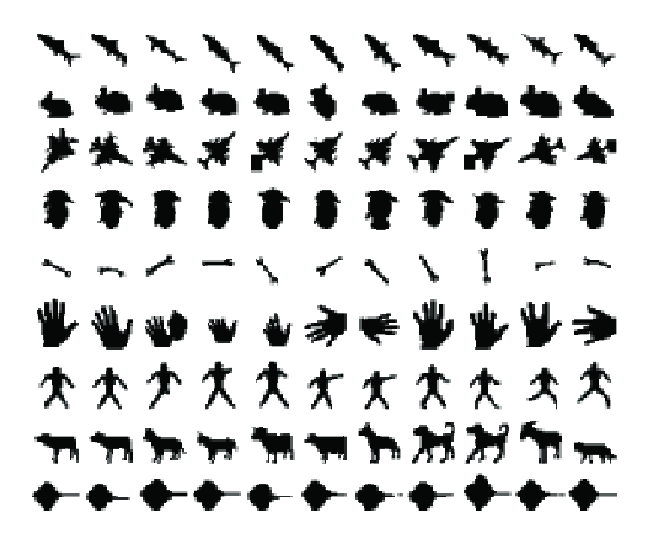
\includegraphics[width=0.5\textwidth]{db.eps}
\end{figure}

\begin{figure}[h!]
	\caption{\label{fig:db2} Amostras de formas da base de imagens Kimia-216.}
	\centering
	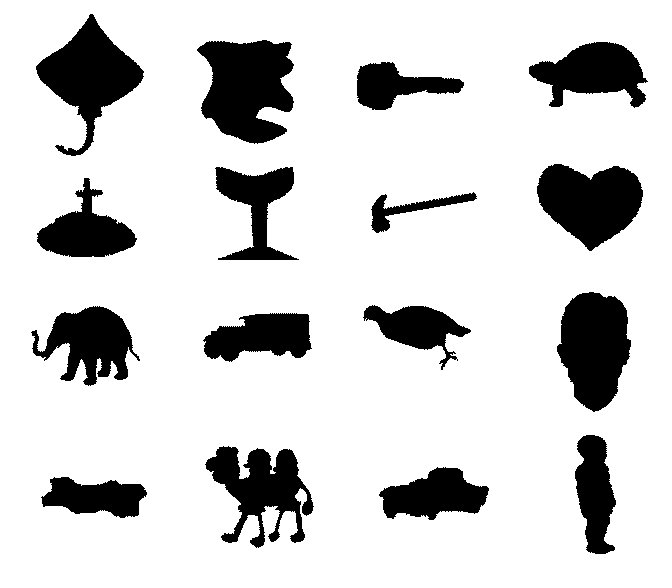
\includegraphics[width=0.5\textwidth]{Dataset.jpg}
\end{figure}

\begin{figure}[h!]
	\caption{\label{fig:db3} Amostras de formas da base de imagens MPEG-7.}
	\centering
	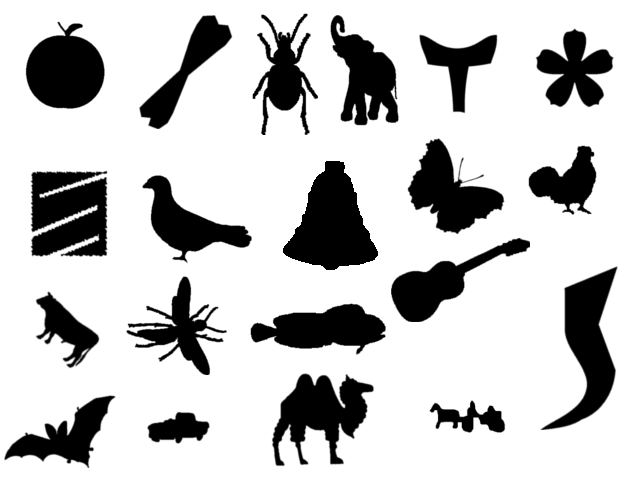
\includegraphics[width=0.5\textwidth]{mpeg7.png}
\end{figure}

Exemplares extraídos da base pública de imagens de folhas intitulada Flavia \cite{4458016} são exibidos na Figura \ref{fig:leaves}. Esta base, composta de  $1907$ imagens de folhas de $32$ espécies distintas, tem sido extensivamente utilizada em trabalhos recentes para testes de métodos de reconhecimento automático de espécies de plantas \cite{wang2015march,quteprints78723,Quadri:2015,Chaki201561}. A base Flavia é bastante desafiadora pois, além de ser desbalanceada, ou seja,  conter classes com quantidades distintas de folhas, ela ainda apresenta espécies com grande variabilidade intra classe e pequena variabilidade entre classes.

\begin{figure}[!ht]
	\caption{\label{fig:leaves} Trinta e duas amostras extraídas da base Flavia, que contém $1907$ imagens de folhas de $32$ espécies diferentes. Cada amostra corresponde a uma espécie.}
	\centering
	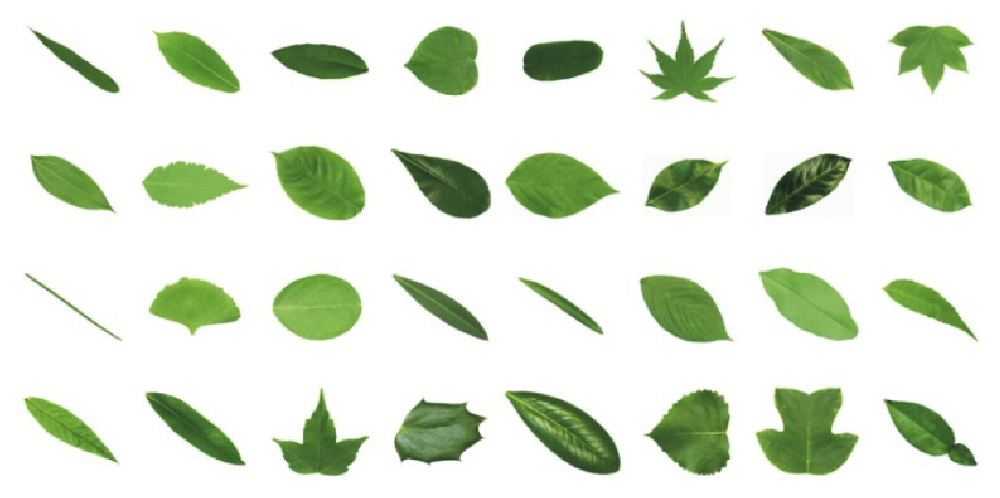
\includegraphics[width= 0.6\textwidth]{folhas.eps}
\end{figure}

\textcolor{red}{
\section{Extração de características\label{sec:EA}}
Aqui vou comentar os dois métodos de extração de características no qual vou aplicar a metodologia (IDSC e NMBE).
Vou também comentar como será feita a avaliação da 
validade do método proposto (comparação do desempenho com o ajuste de parâmetros obtido através de otimização e valores dos parâmetros sugeridos na literatura.
e por valores propostos na literatura.
}

\section{Avaliação do descritor}

Nesta tese, o desempenho do descritor customizado é avaliado qualitativa e quantitativamente. Na avaliação qualitativa, dois algoritmos de visualização de dados são utilizados: o mapa auto-organizável de Kohonen \cite{Kohonen:2001} e o \textit{escalonamento multidimensional} \cite{cox:2000}. Na avaliação quantitativa,  são analisadas as métricas de avaliação Precisão e Revocação \cite{Paula:2013} obtidas em experimentos de classificação supervisionada, a medida \textit{Bulls-eye} \cite{Alajlan20117,Ling:2007:SCU:1191552.1191806}, classicamente utilizada em experimentos de recuperação de formas (\ac{CBIR}) e a medida de avaliação de agrupamentos \textit{silhouette} \cite{Rousseeuw:1987}. 

Para fins de comparação,  as avaliações de desempenho qualitativa e quantitativa foram realizadas com as versões dos descritores otimizados pelo método proposto e não otimizados, seja por escolha aleatória dos parâmetros ou por meio de ajuste apresentado em \cite{Costa:1997}.

\subsection{Visualização dos dados}

Algoritmos de visualização de dados produzem projeções bidimensionais das descrições das formas da base de folhas, provendo uma representação gráfica que possibilita a análise da qualidade dos agrupamentos. Assim, consegue-se inferir o quão eficaz o descritor é em organizar espacialmente as formas. Os métodos de visualização empregados neste trabalho são o mapa auto-organizável de Kohonen \cite{Kohonen:2001} e o \textit{escalonamento multidimensional (\ac{MDS})} \cite{cox:2000}.

A Figura \ref{fig:projkimia99} mostra a matriz-U para formas da base MPEG-7 CE-Shape-1 data set \cite{855850}. A imagem central é o resultado do processamento de todas as imagens da base descrita pela \ac{NMBE} otimizada. As quatro imagens dos cantos são detalhes da imagem central. 

\begin{figure}[h]
\caption{\label{fig:projkimia99} Matrizes-U para as formas da base MPEG7 CE-Shape-1.}
\centering
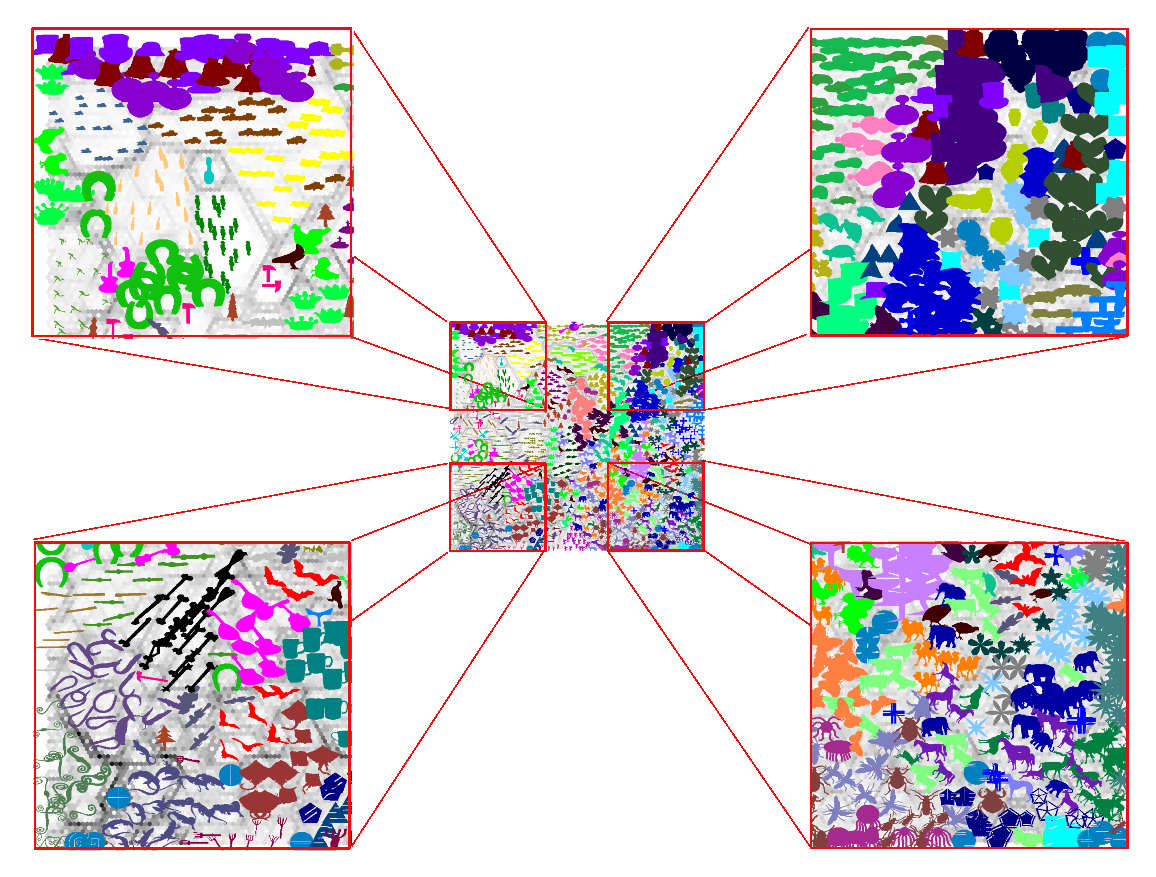
\includegraphics[width=0.8\textwidth]{fig3.eps}
\end{figure}

Essa ferramenta de visualização identifica quão bem a \ac{NMBE} descreve detalhes sutis das formas de um mesmo agrupamento e de diferentes agrupamentos. Nas imagens de detalhes se observa que as fronteiras entre os agrupamentos (cor cinza) estão evidentes e separam agrupamentos bem definidos. Nesta tese assumimos que agrupamentos bem definidos são aqueles com menor distância dentro das classes e maior distância entre classes.  

As projeções \textit{\ac{MDS}} da Figura \ref{fig:optimization_result} ilustram como os agrupamentos evoluem à medida que o algoritmo \ac{DE} busca os parâmetros otimizados do descritor (\ac{NMBE}). As amostras de formas exibidas pertencem à base Kimia-99 \cite{Sebastian:2004}, a qual contém $99$ imagens. Neste trabalho, aplicamos técnicas de aprendizagem (\textit{manifold learning}) para produzir as projeções \ac{MDS} do descritor \ac{NMBE} otimizado utilizando o algoritmo \ac{DE}.  A Figura \ref{fig:optimization_result} demonstra que à medida que os valores de \ac{MAD} decrescem, as distâncias entre as classes aumentam e consequentemente os agrupamentos das classes se tornam mais evidentes. Nesta figura, quando o método de otimização converge, ou seja \ac{MAD} alcança o menor valor,   os únicos agrupamentos que não estão bem separados são aqueles relacionados às formas de animais quadrúpedes e de mãos.

\begin{figure}[h]
\caption{\label{fig:optimization_result} Projeções do escalonamento multidimensional das formas da base Kimia-99 \citeonline{Sebastian:2004}. As imagens mostram como os agrupamentos evoluem ao longo do processo de otimização (\ac{DE}), assim como os valores de \ac{MAD} e $R^2$.}
\centering
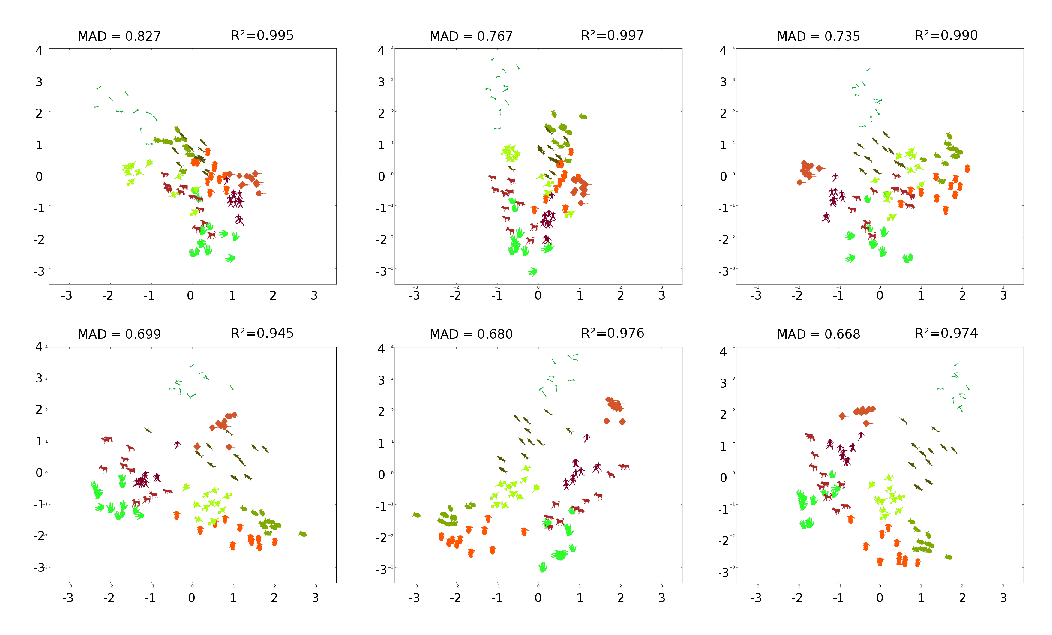
\includegraphics[width = \textwidth]{fig4.eps}
\end{figure}

\subsection{Recuperação de formas}

Visando avaliar o desempenho dos descritores de  forma, foram realizados experimentos de recuperação de imagens pelo conteúdo em duas bases de imagens de formas binárias (Kimia-99 e MPEG-7 CE-Shape-1) e uma  base de folhas (Flavia). 

A  Figura \ref{fig:metodo_cbir} ilustra a metodologia dos experimentos de recuperação de formas.  Primeiramente realiza-se a extração de características das formas da base de imagens com o método de descrição sob avaliação. Desse processo, resulta uma base de dados com os vetores de características associados às formas, que serão utilizados no experimento. 

O mesmo processo de extração de características é aplicado à imagem da forma de consulta. Essa última corresponde ao padrão de entrada ao qual as demais formas da base serão comparadas, através de uma medida de similaridade, a fim de se estabelecer o grau de correspondência existente entre as mesmas. Desta forma, tem-se como resultado a lista das imagens recuperadas na ordem decrescente da similaridade que apresentam em relação à forma de consulta. Todo esse processo é realizado tomando-se cada forma da base de imagens como forma de consulta para realização da recuperação das demais.

Como medida de dissimilaridade nos experimentos \ac{CBIR} com descritores multiescala, empregamos a distância  euclidiana entre os vetores de características das formas. A distância euclidiana entre os vetores $a$ e $b$ de mesma dimensão $n$ é definida como: %${d}_{euclidiana} =  \sum_{i=1}^{N}{({a}_{i}-{b}_{i})}^{2}$,
\begin{equation}
\label{eq:dist_euclidiana}
{d}_{euclidiana} = \sqrt{\sum_{i=1}^{n}{({a}_{i}-{b}_{i})}^{2}},
\end{equation}
em ${a}_{i}$ e ${b}_{i}$ correspondem às $i$-ésimas componentes dos vetores $a$ e $b$, respectivamente.

%As metodologias utilizadas nesses experimentos são as mesmas encontradas em diversos trabalhos de recuperação de formas da literatura.

\begin{figure}[h!]
\caption{\label{fig:metodo_cbir} Metodologia empregada para os experimentos de recuperação de formas pelo conteúdo.}
  \centering
  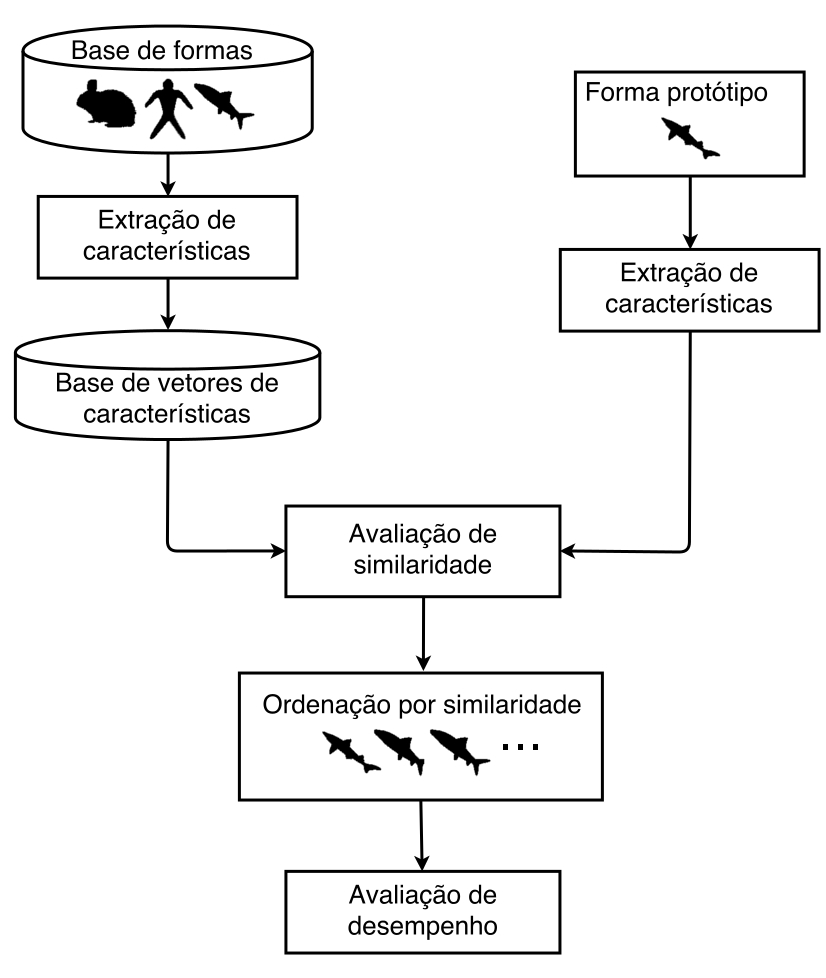
\includegraphics[width=0.6\textwidth]{metodo_cbir.jpg}
\end{figure}

%Com a medida de similaridade avalia-se o grau de correspondência existente entre o vetor de características da forma de consulta e os vetores associados a cada uma das formas da base. 


Na avaliação do desempenho destes experimentos, empregamos duas medidas que são  o número total de acertos por posição recuperada e a medida \textit{Bulls-eye} \cite{Ling:2007:SCU:1191552.1191806,Latecki2000}.
A primeira medida consiste no número total de ocorrências de formas da mesma classe que a forma de consulta em cada posição recuperada.  Em diversos trabalhos de recuperação de formas pelo conteúdo, o número total de acertos por posição recuperada é calculado para a base Kimia-99 \cite{Bernier:2003}. Para esta base, que contém 99 formas igualmente distribuídas em 9 classes, ou seja é uma base balanceada, são realizadas 99 recuperações das 11 formas mais similares à imagem de consulta. Como resultado espera-se obter um total de 99 formas recuperadas corretamente para cada posição recuperada.

A medida  \textit{Bulls-eye} \cite{Latecki2000} originalmente foi definida para avaliar o desempenho de descritores de forma em experimentos \ac{CBIR} com a base de imagens MPEG-7, podendo ser adaptada para outras bases. Esta medida também é utilizada na literatura para a comparação de diferentes métodos de recuperação de formas. Seu cálculo  para a base MPEG-7 CE-Shape-1 é obtido da seguinte maneira: tomando-se cada forma dessa base de imagens como elemento de consulta, contabiliza-se o número de recuperações pertencentes à mesma classe da forma de consulta dentre as $40$ primeiras posições recuperadas. Como resultado calcula-se a percentagem da quantidade máxima de recuperações corretas possíveis de se alcançar, sendo esta última quantidade $28000 = 1400\text{ formas} \times 20\text{ recuperações corretas por forma}$.


%
% Considerando uma base de imagens, cujo número de elementos é dado por $N_B$, com a mesma quantidade de objetos em todas suas classes. O número de classes é representado por $N_C$ e o de elementos de determinada classe é denotado por $N_E$.

Em caso de bases de imagens balanceadas, ou seja, com a mesma quantidade de objetos em todas suas classes, pode-se definir $N_B$ como o número de imagens da base e $N_C$ como o número de elementos de uma determinada classe. Sendo assim, ao realizar o experimento \ac{CBIR}, recupera-se as $2N_C$ imagens mais semelhantes e contabiliza-se quantas foram recuperadas da mesma classe da imagem usada na consulta, sendo esse processo executado para todas $N_B$ imagens da base. O número de imagens recuperadas da mesma classe das imagens testadas em todas iterações é denotado por $N_A$, ou seja, a quantidade de acertos.
Assim a medida \textit{Bulls-eye} ($B_e$) é definida por: %$BE=\frac{Q_A}{N_B N_C}$.
\begin{equation} 
\label{eq:Bulls-eye}
B_e=\frac{N_A}{N_B N_C}.
\end{equation}

O teste \textit{Bulls-eye} apresenta  escores ou valores no intervalo $[0,1]$. Valores próximos a $0$ indicam que os descritores  utilizados no experimento $\ac{CBIR}$ não desempenharam bem na caracterização dos elementos da base em estudo, e valores perto de $1$ indicam  bom desempenho.

\subsection{Classificação supervisionada}

\begin{figure*}[b]
\caption{\label{fig:Classific}
Metodologia de classificação para avaliação de desempenho do descritor otimizado pelo método proposto exibido na Figura.  \ref{fig:Avaliacao}} 
\centering
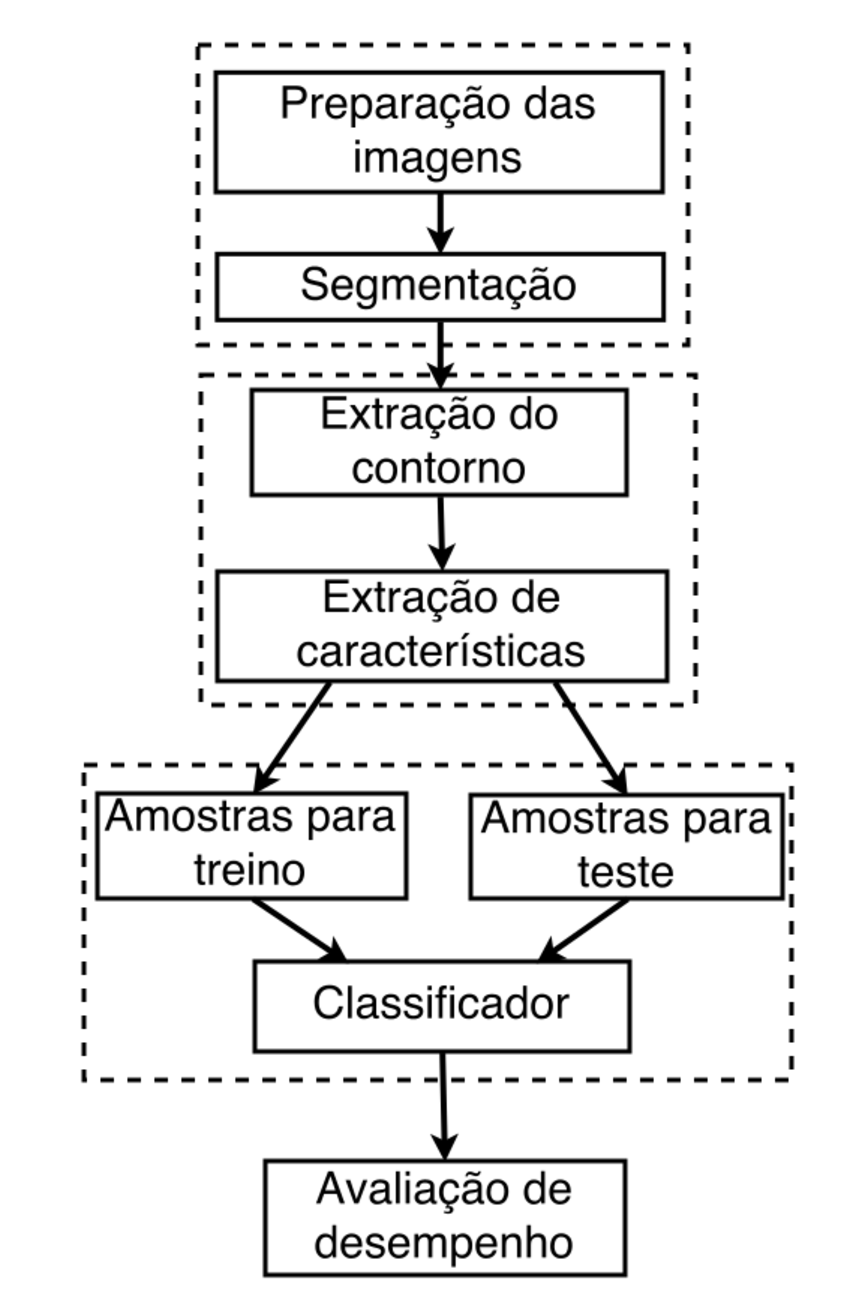
\includegraphics[width=0.4\textwidth]{metodo_classifica.pdf}
\end{figure*}

O procedimento para avaliar o desempenho do descritor multiescala em classificação supervisionada está ilustrado na Figura \ref{fig:Classific}. Para fins de clareza, este procedimento foi dividido em três etapas: pré-processamento, extração de características e a classificação propriamente dita. Detalhamos cada dessas etapas, bem como as sub-etapas a elas relacionadas.

\subsubsection*{Pré-processamento}

A etapa de pré-processamento é aplicada às imagens das folhas da base Flavia, uma vez que as imagens das bases MPEG7-CE e Kimia-99 já encontram-se binarizadas. Essa etapa está dividida em duas sub-etapas: preparação das imagens e segmentação. 

A preparação das imagens elimina os ruídos inerentes ao processo de aquisição das imagens das folhas. Essa sub-etapa é um tratamento preliminar, que é realizado para garantir um bom resultado de segmentação. Esse tratamento preliminar começa com a extração de um dos três canais de cor RGB da imagem, sendo o canal G o que foi extraído para segmentação. A razão dessa escolha é que este canal incorpora boa parte da informação contida nas imagens de interesse, que correspondem apenas a imagens de folhas verdes. 

O próximo passo consiste na aplicação de um filtro bilateral \cite{Gonzalez:2006} às imagens para homogeneizar as intensidades dos pixels.  Além de favorecer a segmentação, este tipo de filtro tem a propriedade de preservar as bordas das formas, que é onde se encontra a informação de interesse para a extração dos atributos (Seção \ref{sec:EA}). 

Finalizando o pré-processamento, a segmentação por limiar \cite{Gonzalez:2006} é aplicada às imagens tratadas, estando assim as imagens preparadas para a próxima etapa, que é a extração de características.

\subsubsection*{Extração de características}

Antes da etapa de extração de características, obtém-se as coordenadas paramétricas do contorno das formas segmentadas através do seguidor de bordas proposto por \citeonline{Suzuki198532}.
Os descritores são então obtidos, a partir dos contornos das formas, pelo método de extração de atributos descrito na Seção \ref{sec:EA}. 

\subsubsection*{Classificação}

Para a etapa de classificação, os descritores  obtidos na etapa anterior são divididos em grupos de amostras de teste/treino, sendo o método utilizado para geração desses grupos o k-fold (k = 10) \cite{Webb:2002}. 

Para cada grupo de testes e treino, os descritores são  transformados pelo discriminante linear de Fisher \cite{Webb:2002}, para melhorar a separação inter classes e a coesão intra classe, e pela \ac{PCA}, para  descorrelacioná-los. Cabe aqui salientar que as matrizes utilizadas nessas transformações são obtidas apenas considerando as amostras selecionadas para treino dos classificadores.

A última sub-etapa da classificação envolve a realização da validação cruzada, com os $10$ grupos de teste e treino gerados \cite{Webb:2002}, para quatro classificadores estatísticos: \ac{NB} \cite{Fukunaga:1990}, \ac{kNN}, \cite{Fukunaga:1990,Webb:2002}, \ac{LDA} \cite{Webb:2002} e \ac{QDA} \cite{Fukunaga:1990}. 

O \ac{LDA} e o \ac{QDA} são classificadores que assumem modelo Gaussiano multivariado dos dados. Como os nomes sugerem,  estes classificadores estabelecem superfícies de decisão lineares e quadráticas, respectivamente. Por serem paramétricos apresentam soluções fechadas, o que os torna simples de serem implementados. Ademais, o \ac{LDA} e o \ac{QDA} são inerentemente adequados para resolução de problemas que envolvam a classificação de múltiplas classes.

Quando se assume, no modelo do classificador \ac{QDA}, que as matrizes de covariância das classes são diagonal e idênticas, que significa assumir classes condicionalmente independentes, o \ac{QDA} se torna o \ac{NB}). 

Apesar da aparente simplicidade, o classificador \ac{NB} tem demonstrado desempenho satisfatório em diversas aplicações de reconhecimento de padrões, como a classificação de documentos e a filtragem de spams. Além de sua eficiência computacional, o \ac{NB} requer pequenas quantidades de amostras de treino para estimação de seus parâmetros.

O \ac{kNN} é um classificador não paramétrico, comumente utilizado em situações onde a superfície de decisão entre classes é irregular. Por não ser paramétrico, este classificador não constrói um modelo de distribuição das classes a partir de amostras de treino, mas infere a classe das amostras de teste diretamente a partir das de treino. Desta forma, a classificação se dá por votação entre os $k$ vizinhos mais próximos à amostra de teste da qual se deseja inferir a classe, sendo atribuído o rótulo da classe que é a mais representativa entre os $k$ pontos vizinhos consultados. Em geral, a métrica de distância utilizada é a euclidiana, porém outras métricas podem ser empregadas. A desvantagem do \ac{kNN} é que a escolha do parâmetro $k$ é extremamente dependente dos dados. Em geral, valores grandes de $k$ aumentam a robustez do classificador a ruídos, mas torna as fronteiras de decisão entre as classes menos evidente.

A partir dos resultados de $100$ execuções da validação cruzada, foram calculados os valores médios e os desvios padrão das medidas clássicas de desempenho Precisão e Revocação.

%\subsection{Avaliação quantitativa de agrupamentos}

%A \textit{silhouette} média por classe avalia tanto a coesão como a separação das classes através da distância entre os vetores de características.




%A avaliação de similaridade entre formas a partir de medidas de divergência requer que as informações das assinaturas, abordadas na Seção \ref{sec:Assinatura} do Capítulo \ref{chap:contour}, sejam tratadas como variáveis aleatórias e que suas distribuições de probabilidade sejam estimadas. 

%A  Figura \ref{fig:metodo_distancia} ilustra como divergentes podem ser aplicados na avaliação da similaridade entre duas formas A e B. No método em questão, as distribuições de probabilidade de quatro assinaturas distintas dos contornos das formas são estimadas, através de histogramas, para em seguida se calcular as medidas de divergência. Uma medida de similaridade é então obtida  a partir da média ponderada das medidas de divergência.

\begin{comment}
\subsection{Visualização de dados}

A Figura \ref{fig:metodo_4} ilustra o método que empregamos na avaliação da capacidade discriminativa dos descritores de formas através das técnicas de visualização dos dados apresentadas.

\begin{figure}[h!]
  \caption{\label{fig:metodo_4} Método de avaliação de descritores multiescala do contorno de formas. (a) Base de imagens. (b) Extração de características. (c) Descritores de formas. (d) Análise de similaridade a partir da matriz-U. (e) Avaliação de agrupamentos a partir da medida silhouette.}
  \centering
  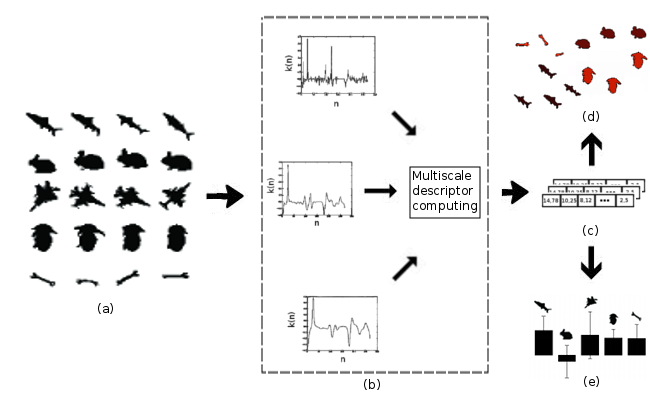
\includegraphics[width=\textwidth]{metodo_v4.png}
\end{figure}

O primeiro passo consiste em realizar a extração de características num conjunto de formas binárias rotuladas (Figura \ref{fig:metodo_4}a e Figura \ref{fig:metodo_4}b) com o método de descrição sob análise. Como resultado temos um conjunto de descritores, ou vetores de características, das referidas formas (Figura \ref{fig:metodo_4}c). 

A avaliação de qualidade dos descritores se dá qualitativamente e quantitativamente. Na avaliação qualitativa (Figura \ref{fig:metodo_4}d) utilizamos a rede auto-organizável de Kohonen para obtenção da matriz de distâncias unificada, ou matriz-U. Essa última é empregada como ferramenta de visualização dos dados, o que possibilita identificar como o método de descrição sob avaliação agrupa as formas. 

Na avaliação quantitativa (Figura \ref{fig:metodo_4}e) utilizamos os rótulos e os vetores de características das formas para calculamos a medida de avaliação de agrupamentos \emph{Silhouette} \cite{Rousseeuw:1987}. Valores médios dessa medida, por classe de formas, indica a habilidade dos descritores em discriminar formas que pertençam a classes distintas e de agrupar formas que pertençam a uma mesma classe.
\end{comment}

\begin{comment}
Although the curvature signal is a sensitive signature to local features of the shape contour, such as concavity and spatial location of salient points, its low noise immunity limits it for shape description application. Thus, it is recommended to smooth  the contour before calculating the curvature signal in order to yield a more robust representation, albeit losing information \citep{Cesar:1996}. A usual smoothing strategy is the discrete convolution of $z[n]$ with a Gaussian kernel, as follows

\begin{equation}
z_{\sigma}[n] = \sum_{i=1}^{N}z[i]g_{\sigma}[n-i],
\label{eq:zsigma}
\end{equation}

\noindent where $g_{\sigma}[n]$ is a Gaussian kernel filter and
$\sigma$ stands for the scale parameter for smoothing control. The Gaussian filter $g_{\sigma}[n]$ is given by\\ 

\begin{equation}
g_{\sigma}[n] = \frac{1}{\sigma\sqrt{2\pi}}e^{-n^{2}/2\sigma^{2}}. 
\end{equation}


It is well-known that this filtering process modifies the amplitude of the respective spectral representation of the contour in such a way that the contour tends to shrink as the kernel scale parameter decreases \citep{Cesar:1996,Costa:1997}. One strategy to avoid such effect is to normalize the smoothed contour as

\begin{equation}
\breve{z}_{\sigma}[n] = \frac{P}{P_{\sigma}}z_{\sigma}[n],
\end{equation}

\noindent where $P$ and $P_{\sigma}$ are the perimeters of the non-smoothed and smoothed contours, respectively.

By replacing $k[n]$ by $k_{\sigma}[n]$ and $z[n]$ by $\breve{z}_{\sigma} [n]$ in equations \ref{eq:ebe} and \ref{eq:kn}, and calculating these equations for $M$ different smoothing scale factors  $\sigma = (\sigma_{1}\text{, }\sigma_{2}\text{, }\ldots\text{ , }\sigma_{M})$, we obtain a multiscale representation of the bending energy given by:

\begin{equation}
NMBE = (\log{E_{\sigma_{1}}}\text{, }\log{E_{\sigma_{2}}}\text{, }\ldots \text{ , }\log{E_{\sigma_{M}}}).
\label{eq:nmbe}
\end{equation}
\end{comment}


%Os descritores entropia multiescala, apresentado no Capítulo \ref{chap:FUNDA}, e a energia de dobramento multiescala requerem o ajuste dos seguintes parâmetros: o número e os valores dos fatores de escala utilizados na representação das formas. Esse capítulo apresenta um método robusto e versátil para o ajuste desses parâmetros para customizar esses descritores em aplicações de classificação supervisionada e não supervisionada.   
